\documentclass[12pt]{report}
\usepackage[utf8]{inputenc}
\usepackage[russian]{babel}
%\usepackage[14pt]{extsizes}
\usepackage{listings}

% Для листинга кода:
\lstset{ %
language=go,                 % выбор языка для подсветки 
basicstyle=\small\sffamily, % размер и начертание шрифта для подсветки кода
numbers=left,               % где поставить нумерацию строк (слева\справа)
numberstyle=\tiny,           % размер шрифта для номеров строк
stepnumber=1,                   % размер шага между двумя номерами строк
numbersep=5pt,                % как далеко отстоят номера строк от подсвечиваемого кода
showspaces=false,            % показывать или нет пробелы специальными отступами
showstringspaces=false,      % показывать или нет пробелы в строках
showtabs=false,             % показывать или нет табуляцию в строках            
tabsize=2,                 % размер табуляции по умолчанию равен 2 пробелам
captionpos=t,              % позиция заголовка вверху [t] или внизу [b] 
breaklines=true,           % автоматически переносить строки (да\нет)
breakatwhitespace=false, % переносить строки только если есть пробел
escapeinside={\#*}{*)}   % если нужно добавить комментарии в коде
}

% Для измененных титулов глав:
\usepackage{titlesec, blindtext, color} % подключаем нужные пакеты
\definecolor{gray75}{gray}{0.75} % определяем цвет
\newcommand{\hsp}{\hspace{20pt}} % длина линии в 20pt
% titleformat определяет стиль
\titleformat{\chapter}[hang]{\Huge\bfseries}{\thechapter\hsp\textcolor{gray75}{|}\hsp}{0pt}{\Huge\bfseries}

%отступы по краям
\usepackage{geometry}
\geometry{verbose, a4paper,tmargin=2cm, bmargin=2cm, rmargin=1.5cm, lmargin = 3cm}
% межстрочный интервал
\usepackage{setspace}
\onehalfspacing
\usepackage{float}
% plot
\usepackage{pgfplots}
\usepackage{filecontents}
\usepackage{amsmath}
\usepackage{tikz,pgfplots}
\usetikzlibrary{datavisualization}
\usetikzlibrary{datavisualization.formats.functions}

\usepackage{graphicx}
\graphicspath{{src/}}
\DeclareGraphicsExtensions{.pdf,.png,.jpg}
\usepackage{amsmath}
\usepackage{geometry}
\geometry{verbose, a4paper,tmargin=2cm, bmargin=2cm, rmargin=1.5cm, lmargin = 3cm}
\usepackage{indentfirst}
\setlength{\parindent}{1.4cm}

\usepackage{titlesec}
\titlespacing{\chapter}{0pt}{12pt plus 4pt minus 2pt}{0pt}

\begin{filecontents}{timeHash.dat}
	100000 5.187925
	500000 30.5863
	700000 41.655
	1000000 58.1547
\end{filecontents}

\begin{document}
%\def\chaptername{} % убирает "Глава"
\begin{titlepage}
	\centering
	{\scshape\LARGE МГТУ им. Баумана \par}
	\vspace{3cm}
	{\scshape\Large Рубежный контроль №1\par}
	\vspace{0.5cm}	
	{\scshape\Large По курсу: "Анализ алгоритмов"\par}
	\vspace{1.5cm}
	{\huge\bfseries Эффективная реализация алгоритма\par}
	\vspace{2cm}
	\Large Работу выполнил: Мокеев Даниил, ИУ7-54\par
	\vspace{0.5cm}
	\Large Преподаватели:  Волкова Л.Л., Строганов Ю.В.\par

	\vfill
	\large \textit {Москва, 2019} \par
\end{titlepage}

\tableofcontents

\newpage
\chapter*{Задание}
\addcontentsline{toc}{chapter}{Введение}

Задание существует таблица, содержащая следующие сущности: idPerson, idArticle, EntityTag (Рис. \ref{exp}). Необходимо выбрать все idPerson, которые работали над одним параграфом.
\begin{figure}[h!]
	\begin{center}
		\begin{tabular}{|c c c|} 
			\hline
			idPerson  & idEntity & EntityTag\\ [0.5ex] 
			\hline\hline
			1 & 3 & "Event"  \\
			\hline
			2 & 6 & "Person"\\
			\hline
			... & ... & ... \\
			\hline
		\end{tabular}
	\end{center}
	\caption{Результаты эксперемента}
	\label{exp}
\end{figure}

Задачи данной лабораторной работы:
\begin{itemize}
	\item Разработать эффективный алгоритм решения задачи;
	\item сравнить его с полным перебором.
\end{itemize}


\chapter{Аналитическая часть}
Для решения данной задачи было решено использовать структуру данных - хэш-таблицу

\section{Хэш-таблицы} 
Существуют два основных варианта хеш-таблиц: с цепочками и открытой адресацией. Хеш-таблица содержит некоторый массив $H$, элементы которого есть пары (хеш-таблица с открытой адресацией) или списки пар (хеш-таблица с цепочками).

Ситуация, когда для различных ключей получается одно и то же хеш-значение, называется коллизией. Такие события не так уж и редки — например, при вставке в хеш-таблицу размером 365 ячеек всего лишь 23 элементов вероятность коллизии уже превысит 50 % (если каждый элемент может равновероятно попасть в любую ячейку) — см. парадокс дней рождения. Поэтому механизм разрешения коллизий — важная составляющая любой хеш-таблицы.

В некоторых специальных случаях удаётся избежать коллизий вообще. Например, если все ключи элементов известны заранее (или очень редко меняются), то для них можно найти некоторую совершенную хеш-функцию, которая распределит их по ячейкам хеш-таблицы без коллизий. Хеш-таблицы, использующие подобные хеш-функции, не нуждаются в механизме разрешения коллизий, и называются хеш-таблицами с прямой адресацией.

Число хранимых элементов, делённое на размер массива $H$ (число возможных значений хеш-функции), называется коэффициентом заполнения хеш-таблицы (load factor) и является важным параметром, от которого зависит среднее время выполнения операций. 
\section{Метод цепочек}
Каждая ячейка массива H является указателем на связный список (цепочку) пар ключ-значение, соответствующих одному и тому же хеш-значению ключа. Коллизии просто приводят к тому, что появляются цепочки длиной более одного элемента.

Операции поиска или удаления элемента требуют просмотра всех элементов соответствующей ему цепочки, чтобы найти в ней элемент с заданным ключом. Для добавления элемента нужно добавить элемент в конец или начало соответствующего списка и в случае, если коэффициент заполнения станет слишком велик, увеличить размер массива H и перестроить таблицу.

При предположении, что каждый элемент может попасть в любую позицию таблицы H с равной вероятностью и независимо от того, куда попал любой другой элемент, среднее время работы операции поиска элемента составляет O(1 + $\alpha$), где $\alpha$ — коэффициент заполнения таблицы.

\chapter{Конструкторская часть}
В данном разделе будут рассмотрены основные требования к программе.

\section{Требования к программе}
\textbf{Требования к вводу:}
\begin{itemize}
	\item Заранее известно сколько сущностей находится в таблице;
	\item cущности располагаются в таблице с небольшим разбросом.
\end{itemize}

\textbf{Требования к программе:}
\begin{itemize}
	\item Алгоритм возвращает таблицу всех людей, работавших с одним параграфом.
\end{itemize}


\section*{Вывод}
\addcontentsline{toc}{section}{Вывод}
В данном разделе были рассмотрены требования к программе.


\chapter{Технологическая часть}

\section{Выбор ЯП}
В качестве языка программирования был выбран golang.
Время работы алгоритмов было замерено с помощью time. 
\section{Сведения о модулях программы}
Программа состоит из:
\begin{itemize}
	\item main.go- главный файл программы, в котором располагается точка входа в программу.
	\item perebor.go - файл содержащий функции измерения времени.
\end{itemize}
\section{Листинг кода алгоритмов}
В данном разделе будут приведены листинги кода полного перебора всех решений (Листинг \ref{brute}) и реализации муравьиного алгоритма (Листинг \ref{hash})
\begin{lstlisting}[label=brute,caption = Перебор всех возможных вариантов, language = go]

func get_articles_brute(ids_person, ids_entity []int, amount int) [][]int{
	articles := make([][]int, 0)
	for i:=0; i<amount; i++{
		articles[i] = make([]int, 0)
	}
	for i:=0; i<len(ids_person); i++{
		tmp := make([]int, 0)
		tmp = append(tmp, 0)
		for j:=0; j<len(ids_person); j++{
			if ids_entity[j] == ids_entity[j]{
			tmp = append(tmp, j)
		}		
		}
		articles = append(articles, tmp)
	}
	return articles
}
\end{lstlisting}

\begin{lstlisting}[label=hash,caption = Муравьиный алгоритм, language = go]

func get_articles_hash(ids_person, ids_entity []int, amount int) [][]int{
	articles := make([][]int, amount, amount)
	for i:=0; i<amount; i++{
		articles[i] = make([]int, 0)
	}
	for i:=0; i<amount; i++{
		for j:=0; j<len(ids_entity); j++{
			if ids_entity[j] == i{
				fl := true
				for k:=0; k < len(articles[i]); k++{
					if ids_person[j] == articles[i][k]{
						fl=false
					}
				}
				if fl{
					articles[i] = append(articles[i], ids_person[j])
				}
			}		
		}
	}
	return articles
} 
\end{lstlisting}
\section*{Вывод}
\addcontentsline{toc}{section}{Вывод}
В данном разделе были рассмотрены основные сведения о модулях программы и листинг кода алгоритмов.

\chapter{Исследовательская часть}
В даннном разделе будет проведен сравнительный временной анализ алгоритмов (Рис. \ref{plot:time}). Замеры времени были произведены на: Intel Core i5-6200U.
\section{Примеры работы}
В данном разделе приведен пример работы программы (Рис. \ref{ris:example})
\begin{figure}[h]
	\centering{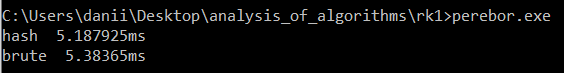
\includegraphics[scale=1.5]{example.png}} 
	\caption{Пример работы программы}
	\label{ris:example}
\end{figure}
\section{Исследование зависимости времени работы алгоритмов от размера графа}
В данном разделе будет приведены результаты сравнения времени работы реализованных алгоритмов в зависимоти от размера Входного файла (Рис. \ref{plot:time}). Время измерено в миллисекундах.
\begin{figure}[!h]
	\begin{tikzpicture}[thick, scale=1.4]
	\begin{axis}[
	axis lines = left,
	xlabel = Количество строк,
	ylabel = Время(миллисекунды),
	legend pos=north west,
	ymajorgrids=true
	]

	\addplot[color=green] table[x index=0, y index=1] {timeHash.dat};
	
	\addlegendentry{Реализованный алгоритм}
	\end{axis}
	\end{tikzpicture}
	\caption{Сравнение параллельного и обычного алгоритмов} \label{plot:time}
\end{figure}
\par

\section{Выводы исследовательского раздела}
Была исследована зависимоть времени работы реализованных алгоритмов от размера входного файла. Реализованный алгоритм показывает линейный темп роста, как и ожидалось. 

\chapter*{Заключение}
\addcontentsline{toc}{chapter}{Заключение}
В ходе рубежного контроля был разработан 
эффективный алгоритм для решения поставленной задачи. Эффективность решения была доказана эксперементально.

\addcontentsline{toc}{chapter}{Список литературы}
\begin{thebibliography}{3}
	\bibitem{diskr} Кормен, Т., Лейзерсон, Ч., Ривест, Р., Штайн, К. Глава 11. Хеш-таблицы. // Алгоритмы: построение и анализ = Introduction to Algorithms / Под ред. И. В. Красикова. — 2-е изд. — М.: Вильямс, 2005. — 1296 с. — ISBN 5-8459-0857-4.
	\bibitem{commi2} Брюс Шнайер. Прикладная криптография. Протоколы, алгоритмы, исходные тексты на языке Си. — М.: Триумф, 2002. — ISBN 5-89392-055-4.
	\bibitem{commi} Дональд Кнут. Искусство программирования. Том 3. Сортировка и поиск = The Art of Computer Programming, vol.3. Sorting and Searching. — 2-е издание. — М.: «Вильямс», 2007. — С. 824. — ISBN 0-201-89685-0.
\end{thebibliography}

\end{document}

